% Space-time diagram of the palindrome machine on abbbba (generated by figs_c3ch03.py): 28 steps.
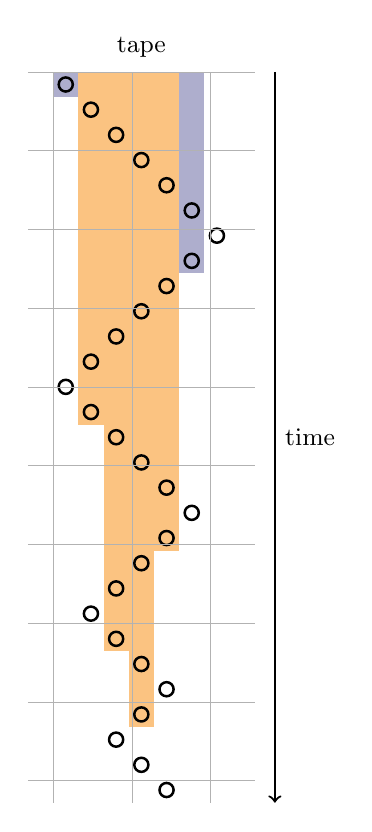
\begin{tikzpicture}[x=0.32cm,y=0.32cm]
\fill[MidnightBlue!35] (0,0) rectangle (1,-1);
\fill[BurntOrange!45] (1,0) rectangle (2,-1);
\fill[BurntOrange!45] (2,0) rectangle (3,-1);
\fill[BurntOrange!45] (3,0) rectangle (4,-1);
\fill[BurntOrange!45] (4,0) rectangle (5,-1);
\fill[MidnightBlue!35] (5,0) rectangle (6,-1);
\draw[black,line width=0.9pt] (0.5,-0.5) circle (0.28);
\fill[BurntOrange!45] (1,-1) rectangle (2,-2);
\fill[BurntOrange!45] (2,-1) rectangle (3,-2);
\fill[BurntOrange!45] (3,-1) rectangle (4,-2);
\fill[BurntOrange!45] (4,-1) rectangle (5,-2);
\fill[MidnightBlue!35] (5,-1) rectangle (6,-2);
\draw[black,line width=0.9pt] (1.5,-1.5) circle (0.28);
\fill[BurntOrange!45] (1,-2) rectangle (2,-3);
\fill[BurntOrange!45] (2,-2) rectangle (3,-3);
\fill[BurntOrange!45] (3,-2) rectangle (4,-3);
\fill[BurntOrange!45] (4,-2) rectangle (5,-3);
\fill[MidnightBlue!35] (5,-2) rectangle (6,-3);
\draw[black,line width=0.9pt] (2.5,-2.5) circle (0.28);
\fill[BurntOrange!45] (1,-3) rectangle (2,-4);
\fill[BurntOrange!45] (2,-3) rectangle (3,-4);
\fill[BurntOrange!45] (3,-3) rectangle (4,-4);
\fill[BurntOrange!45] (4,-3) rectangle (5,-4);
\fill[MidnightBlue!35] (5,-3) rectangle (6,-4);
\draw[black,line width=0.9pt] (3.5,-3.5) circle (0.28);
\fill[BurntOrange!45] (1,-4) rectangle (2,-5);
\fill[BurntOrange!45] (2,-4) rectangle (3,-5);
\fill[BurntOrange!45] (3,-4) rectangle (4,-5);
\fill[BurntOrange!45] (4,-4) rectangle (5,-5);
\fill[MidnightBlue!35] (5,-4) rectangle (6,-5);
\draw[black,line width=0.9pt] (4.5,-4.5) circle (0.28);
\fill[BurntOrange!45] (1,-5) rectangle (2,-6);
\fill[BurntOrange!45] (2,-5) rectangle (3,-6);
\fill[BurntOrange!45] (3,-5) rectangle (4,-6);
\fill[BurntOrange!45] (4,-5) rectangle (5,-6);
\fill[MidnightBlue!35] (5,-5) rectangle (6,-6);
\draw[black,line width=0.9pt] (5.5,-5.5) circle (0.28);
\fill[BurntOrange!45] (1,-6) rectangle (2,-7);
\fill[BurntOrange!45] (2,-6) rectangle (3,-7);
\fill[BurntOrange!45] (3,-6) rectangle (4,-7);
\fill[BurntOrange!45] (4,-6) rectangle (5,-7);
\fill[MidnightBlue!35] (5,-6) rectangle (6,-7);
\draw[black,line width=0.9pt] (6.5,-6.5) circle (0.28);
\fill[BurntOrange!45] (1,-7) rectangle (2,-8);
\fill[BurntOrange!45] (2,-7) rectangle (3,-8);
\fill[BurntOrange!45] (3,-7) rectangle (4,-8);
\fill[BurntOrange!45] (4,-7) rectangle (5,-8);
\fill[MidnightBlue!35] (5,-7) rectangle (6,-8);
\draw[black,line width=0.9pt] (5.5,-7.5) circle (0.28);
\fill[BurntOrange!45] (1,-8) rectangle (2,-9);
\fill[BurntOrange!45] (2,-8) rectangle (3,-9);
\fill[BurntOrange!45] (3,-8) rectangle (4,-9);
\fill[BurntOrange!45] (4,-8) rectangle (5,-9);
\draw[black,line width=0.9pt] (4.5,-8.5) circle (0.28);
\fill[BurntOrange!45] (1,-9) rectangle (2,-10);
\fill[BurntOrange!45] (2,-9) rectangle (3,-10);
\fill[BurntOrange!45] (3,-9) rectangle (4,-10);
\fill[BurntOrange!45] (4,-9) rectangle (5,-10);
\draw[black,line width=0.9pt] (3.5,-9.5) circle (0.28);
\fill[BurntOrange!45] (1,-10) rectangle (2,-11);
\fill[BurntOrange!45] (2,-10) rectangle (3,-11);
\fill[BurntOrange!45] (3,-10) rectangle (4,-11);
\fill[BurntOrange!45] (4,-10) rectangle (5,-11);
\draw[black,line width=0.9pt] (2.5,-10.5) circle (0.28);
\fill[BurntOrange!45] (1,-11) rectangle (2,-12);
\fill[BurntOrange!45] (2,-11) rectangle (3,-12);
\fill[BurntOrange!45] (3,-11) rectangle (4,-12);
\fill[BurntOrange!45] (4,-11) rectangle (5,-12);
\draw[black,line width=0.9pt] (1.5,-11.5) circle (0.28);
\fill[BurntOrange!45] (1,-12) rectangle (2,-13);
\fill[BurntOrange!45] (2,-12) rectangle (3,-13);
\fill[BurntOrange!45] (3,-12) rectangle (4,-13);
\fill[BurntOrange!45] (4,-12) rectangle (5,-13);
\draw[black,line width=0.9pt] (0.5,-12.5) circle (0.28);
\fill[BurntOrange!45] (1,-13) rectangle (2,-14);
\fill[BurntOrange!45] (2,-13) rectangle (3,-14);
\fill[BurntOrange!45] (3,-13) rectangle (4,-14);
\fill[BurntOrange!45] (4,-13) rectangle (5,-14);
\draw[black,line width=0.9pt] (1.5,-13.5) circle (0.28);
\fill[BurntOrange!45] (2,-14) rectangle (3,-15);
\fill[BurntOrange!45] (3,-14) rectangle (4,-15);
\fill[BurntOrange!45] (4,-14) rectangle (5,-15);
\draw[black,line width=0.9pt] (2.5,-14.5) circle (0.28);
\fill[BurntOrange!45] (2,-15) rectangle (3,-16);
\fill[BurntOrange!45] (3,-15) rectangle (4,-16);
\fill[BurntOrange!45] (4,-15) rectangle (5,-16);
\draw[black,line width=0.9pt] (3.5,-15.5) circle (0.28);
\fill[BurntOrange!45] (2,-16) rectangle (3,-17);
\fill[BurntOrange!45] (3,-16) rectangle (4,-17);
\fill[BurntOrange!45] (4,-16) rectangle (5,-17);
\draw[black,line width=0.9pt] (4.5,-16.5) circle (0.28);
\fill[BurntOrange!45] (2,-17) rectangle (3,-18);
\fill[BurntOrange!45] (3,-17) rectangle (4,-18);
\fill[BurntOrange!45] (4,-17) rectangle (5,-18);
\draw[black,line width=0.9pt] (5.5,-17.5) circle (0.28);
\fill[BurntOrange!45] (2,-18) rectangle (3,-19);
\fill[BurntOrange!45] (3,-18) rectangle (4,-19);
\fill[BurntOrange!45] (4,-18) rectangle (5,-19);
\draw[black,line width=0.9pt] (4.5,-18.5) circle (0.28);
\fill[BurntOrange!45] (2,-19) rectangle (3,-20);
\fill[BurntOrange!45] (3,-19) rectangle (4,-20);
\draw[black,line width=0.9pt] (3.5,-19.5) circle (0.28);
\fill[BurntOrange!45] (2,-20) rectangle (3,-21);
\fill[BurntOrange!45] (3,-20) rectangle (4,-21);
\draw[black,line width=0.9pt] (2.5,-20.5) circle (0.28);
\fill[BurntOrange!45] (2,-21) rectangle (3,-22);
\fill[BurntOrange!45] (3,-21) rectangle (4,-22);
\draw[black,line width=0.9pt] (1.5,-21.5) circle (0.28);
\fill[BurntOrange!45] (2,-22) rectangle (3,-23);
\fill[BurntOrange!45] (3,-22) rectangle (4,-23);
\draw[black,line width=0.9pt] (2.5,-22.5) circle (0.28);
\fill[BurntOrange!45] (3,-23) rectangle (4,-24);
\draw[black,line width=0.9pt] (3.5,-23.5) circle (0.28);
\fill[BurntOrange!45] (3,-24) rectangle (4,-25);
\draw[black,line width=0.9pt] (4.5,-24.5) circle (0.28);
\fill[BurntOrange!45] (3,-25) rectangle (4,-26);
\draw[black,line width=0.9pt] (3.5,-25.5) circle (0.28);
\draw[black,line width=0.9pt] (2.5,-26.5) circle (0.28);
\draw[black,line width=0.9pt] (3.5,-27.5) circle (0.28);
\draw[black,line width=0.9pt] (4.5,-28.5) circle (0.28);
\draw[black!30,line width=0.2pt] (-1,0) grid (8,-29);
\draw[->,thick] (8.8,0) -- (8.8,-29) node[midway,right,font=\small] {time};
\node[font=\small,anchor=south] at (3.5,0.2) {tape};
\end{tikzpicture}
